\section{Figures}

\subsection{Side by side images}
%\usepackage[demo]{graphicx}
%\usepackage{subfig}

\begin{figure}[H]
\centering
\parbox{5cm}{
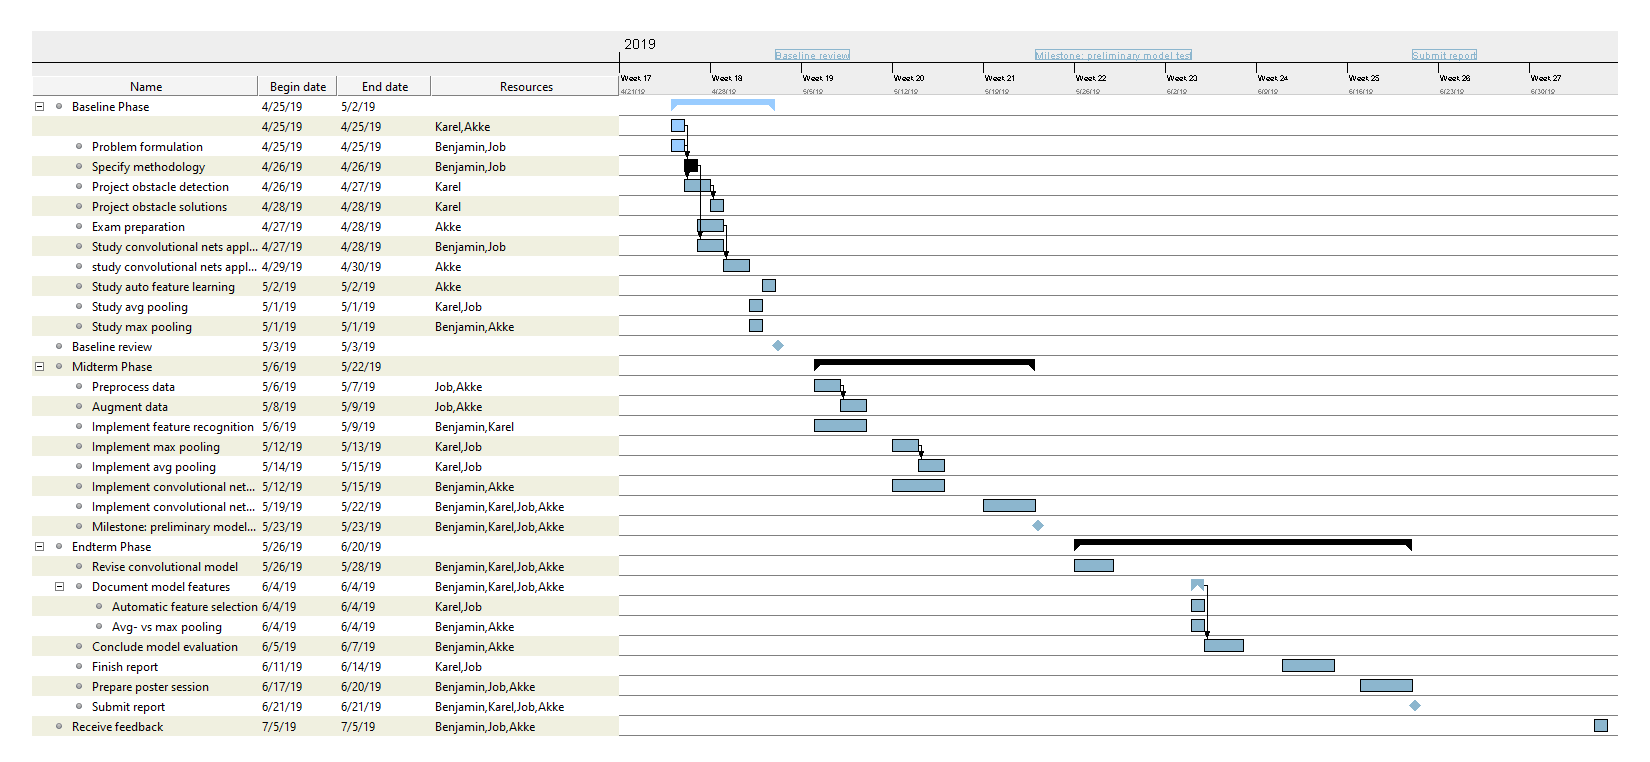
\includegraphics[width=5cm]{images/ganttV4horizontal.png}
\caption{First.}
\label{fig:2figsA}}
\qquad
\begin{minipage}{5cm}
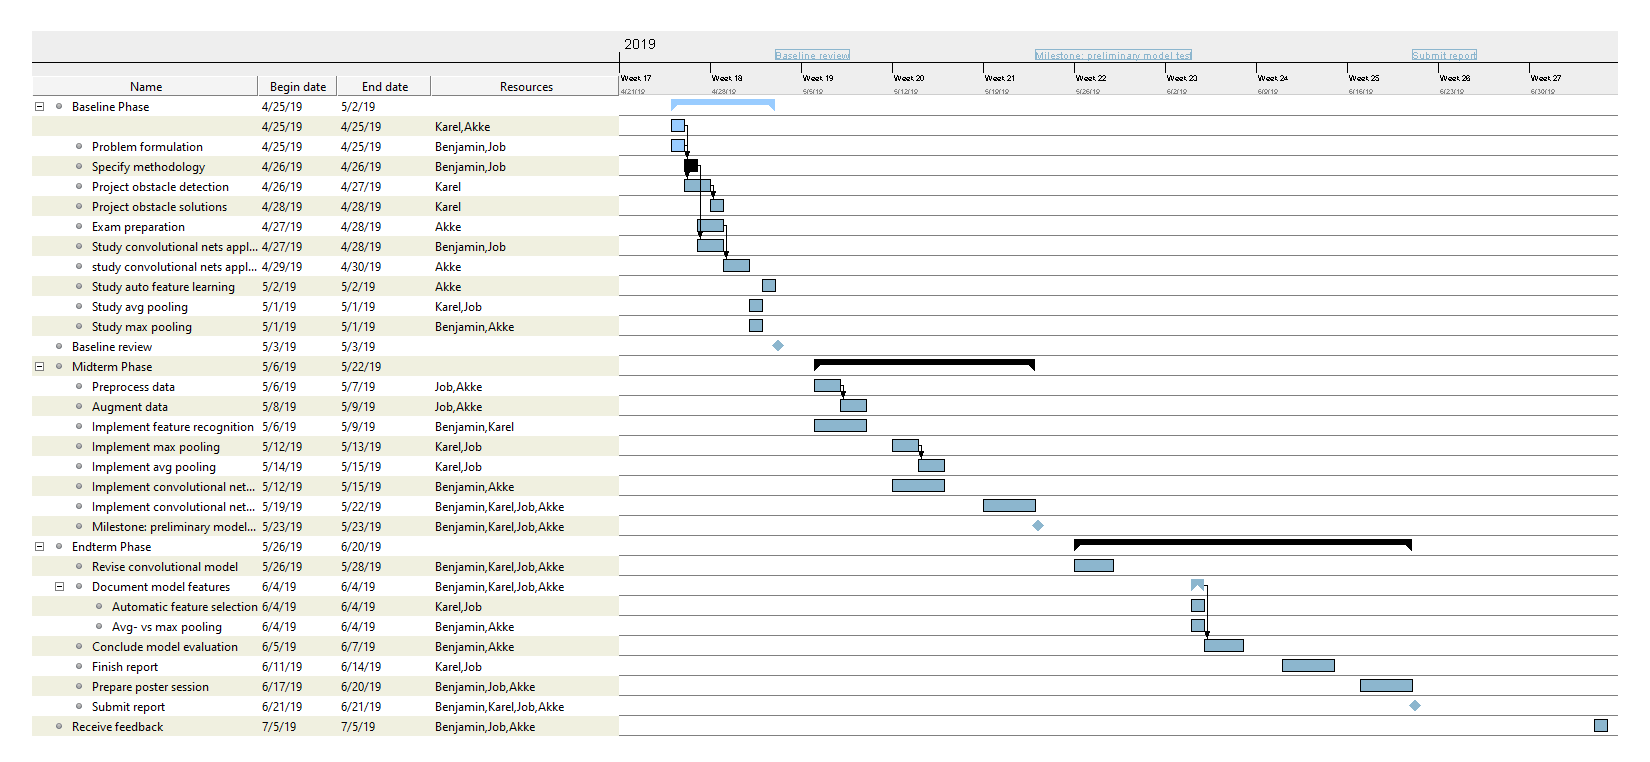
\includegraphics[width=5cm]{images/ganttV4horizontal.png}
\caption{Second.}
\label{fig:2figsB}
\end{minipage}
\end{figure}



%\usepackage{enumitem}
\subsection{Wrap enumeration around figure:}
  {\bfseries Multiple Choice: }% do not use \bf in LaTeX it is deprecated 20+ years ago
  \begin{enumerate}
    \item As shown in the figure. This rock is phaneritic and contains quartz, K-feldspar, and plagioclase in nearly equal amounts. What is it?

    \begin{minipage}{.45\textwidth}
      \begin{enumerate}[label=(\Alph*), itemsep=0pt]% never number things manually!
        \item rhyolite
        \item basa
        \item diorite
        \item ash-flow tuff
        \item  granite
      \end{enumerate}
    \end{minipage}
    \begin{minipage}{.45\textwidth}
      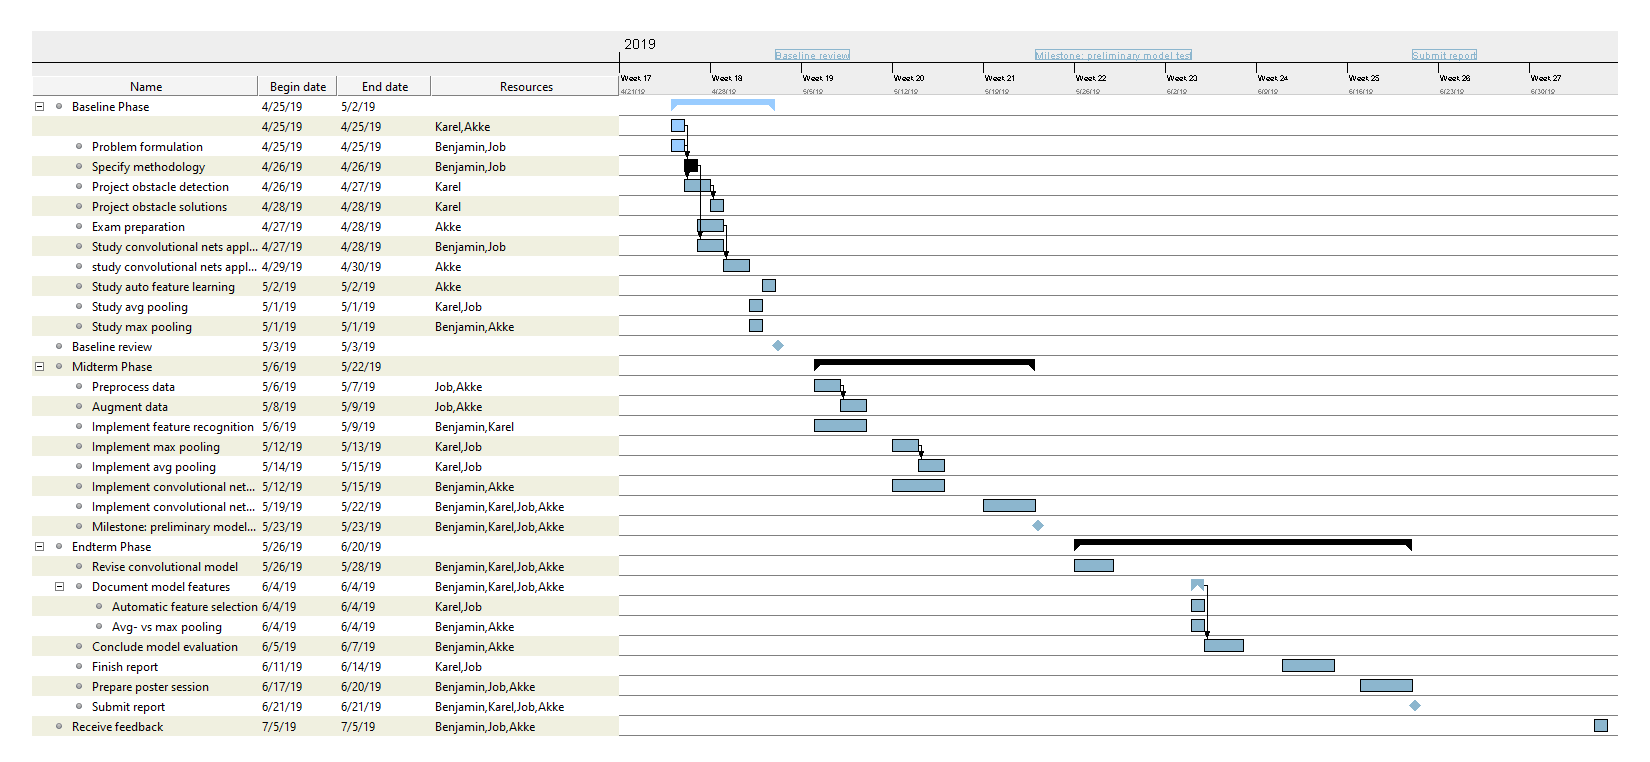
\includegraphics[scale=0.1]{images/ganttV4horizontal.png}
    \end{minipage}
  \end{enumerate}



\subsection{full page horizontal figure with caption}

% \begin{comment}
% % rotate picture attempt 4
% \usepackage{graphicx}
% \usepackage{wrapfig}
% \usepackage{lscape}
% \usepackage{rotating}
% \usepackage{epstopdf}

% \usepackage{graphicx}
% \graphicspath{ {./} }
% \end{comment}

\begin{sidewaysfigure}[ht]
\hspace*{-4cm}   
    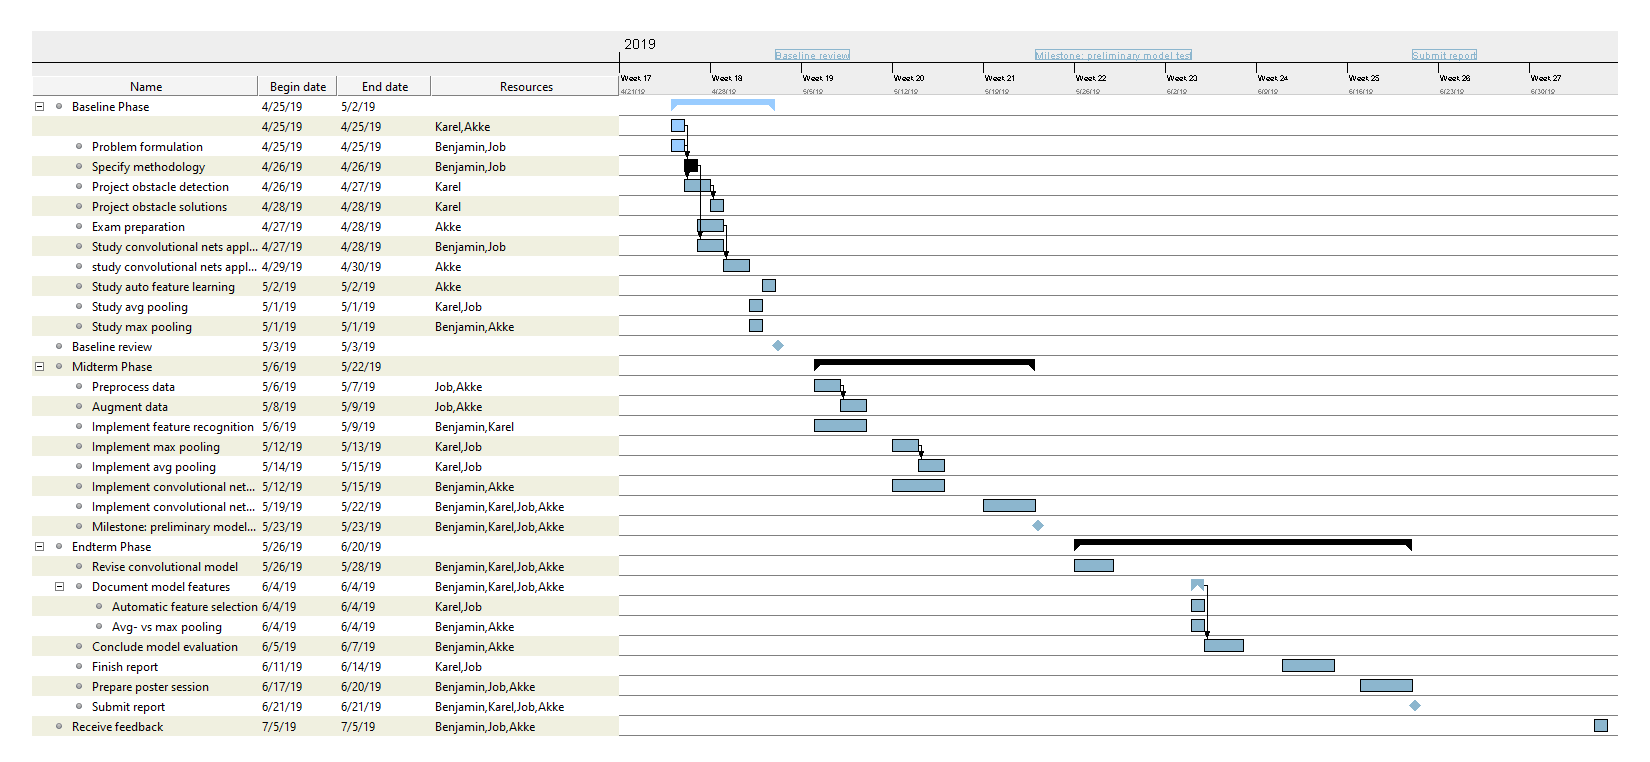
\includegraphics[width = 775pt]{images/ganttV4horizontal.png}
    \caption{Property profile of the diverse library compared to the compound pool.}
    \label{fig:PropProf}
\end{sidewaysfigure}

\subsection{Full page figure}
Figure will fill the page until the edge of the A4 that it encounters.
%\usepackage{pdfpages} % to add a full A4 size gantt chart picture
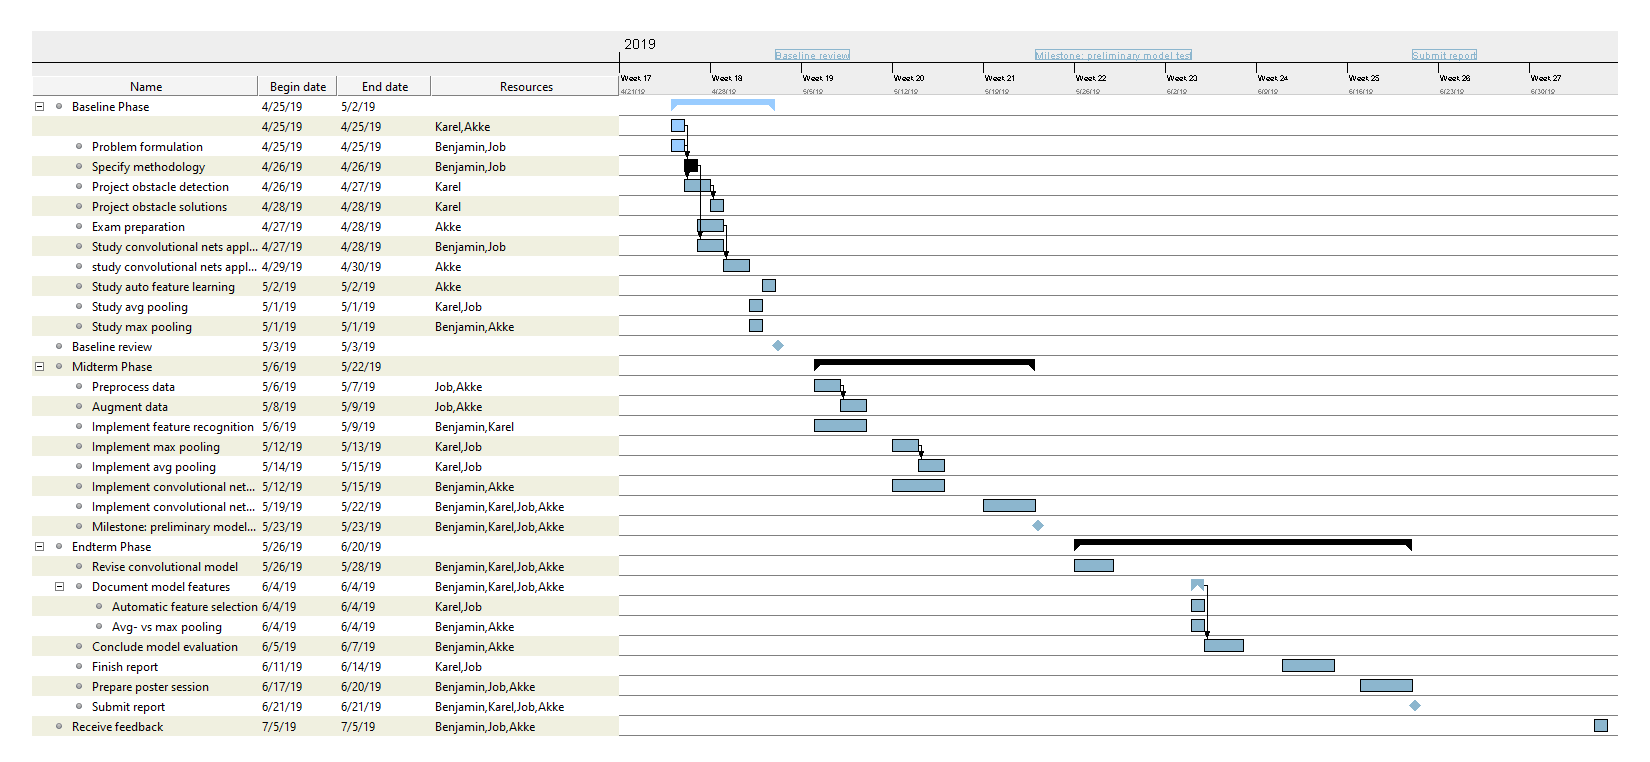
\includepdf{images/ganttV4horizontal.png}

\section{Include eps figure}
Put the following code on the top of main.tex above $begin document$ but below $documentclass{article}$.
\begin{verbatim}
\usepackage{amsmath} % need to be on top for eps files
\usepackage{graphicx}
%set the relative location for eps files
\graphicspath{ {/images/} }
\end{verbatim}

\begin{figure}
    \centering
    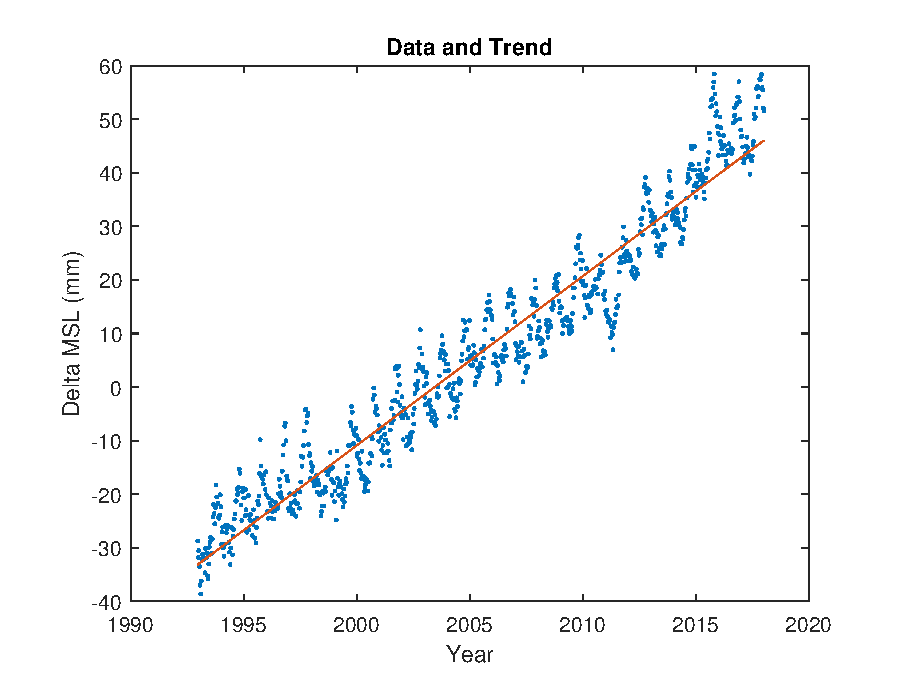
\includegraphics{images/q1a.eps}
    \caption{Trend and bias estimate and visualisation for the seasonal sea-level trend data.}
    \label{fig:plot_q1a}
\end{figure}